% LTeX: enabled=false
\documentclass[aspectratio=169, 11pt]{beamer}
% LTeX: enabled=false

% ---------------------------------------------------------------
% Paquetes
% ---------------------------------------------------------------
\usepackage[utf8]{inputenc}
\usepackage[T1]{fontenc}
\usepackage[spanish, es-nodecimaldot, es-noshorthands, es-tabla]{babel}
\usepackage{times}
\usepackage{amsmath, amssymb}
\usepackage{tabularray}
\usepackage{tikz}
\usetikzlibrary{positioning, fit, backgrounds, calc, arrows.meta, babel}
\usepackage{setspace}               % lo usa el esquema de parámetros corneales del informe
\usepackage{appendixnumberbeamer}   % las diapositivas de respaldo no suman al total
\graphicspath{{img/}}

% ---------------------------------------------------------------
% Estilo (plantilla de las presentaciones de IdS2 y PDS)
% ---------------------------------------------------------------
\usefonttheme{serif}
\definecolor{azul}{HTML}{2C6AA0}
\definecolor{verde}{HTML}{3E8E5E}
\definecolor{gris}{HTML}{F1F1F1}
\definecolor{rojo}{HTML}{B03A2E}

\setbeamercolor{frametitle}{fg=azul}
\setbeamercolor{title}{fg=azul}
\setbeamercolor{structure}{fg=azul}
\setbeamercolor{alerted text}{fg=azul}
\setbeamerfont{alerted text}{series=\bfseries}
\setbeamercolor{block title}{bg=azul, fg=white}
\setbeamercolor{block body}{bg=gris}
\setbeamerfont{frametitle}{series=\bfseries, size=\Large}
\setbeamertemplate{navigation symbols}{}
\setbeamertemplate{itemize items}{\color{azul}\textbullet}
\setbeamertemplate{blocks}[default]

\setlength{\leftmargini}{1.2em}   % listas de primer nivel
\setlength{\leftmarginii}{1.2em}  % listas anidadas

% Pie de página: autores, título corto y número de diapositiva.
% Tres cajas que suman exactamente el ancho de la hoja (0.35 + 0.40 + 0.25).
% Cada línea termina en % para que los saltos de línea no agreguen espacios.
\setbeamercolor{footline}{fg=gray}
\setbeamerfont{footline}{size=\scriptsize}
\setbeamertemplate{footline}{%
    \leavevmode%
    \hbox{%
        \begin{beamercolorbox}[wd=0.35\paperwidth, ht=3ex, dp=1.2ex, left]{footline}%
            \hspace*{1em}Aranda - Wlodeck%
        \end{beamercolorbox}%
        \begin{beamercolorbox}[wd=0.40\paperwidth, ht=3ex, dp=1.2ex, center]{footline}%
            KERALYTIX - Proyecto final integrador%
        \end{beamercolorbox}%
        \begin{beamercolorbox}[wd=0.25\paperwidth, ht=3ex, dp=1.2ex, right]{footline}%
            \insertframenumber\,/\,\inserttotalframenumber\hspace*{1em}%
        \end{beamercolorbox}%
    }%
    \vskip0pt%
}

% Título de cada diapositiva con una línea debajo
\setbeamertemplate{frametitle}{%
    \vspace{0.4em}\insertframetitle\par\vspace{0.2em}{\color{azul}\hrule height 0.6pt}}

% ---------------------------------------------------------------
% Macros propias
% ---------------------------------------------------------------

% Idea clave: caja recta, fondo gris y borde azul
\newcommand{\idea}[1]{%
    \begin{center}
        \setlength{\fboxsep}{5pt}%
        \fcolorbox{azul}{gris}{\parbox{0.9\linewidth}{\centering #1}}
    \end{center}}

% Marca de contenido pendiente (no debe quedar ninguna en la versión final)
\newcommand{\pendiente}[1]{%
    \fcolorbox{rojo}{rojo!5}{\parbox{0.9\linewidth}{\centering\small\color{rojo}%
    \textbf{PENDIENTE}\\ #1}}}

% Estado de un resultado, como pide la consigna: alcanzado, en proceso o pendiente.
% #1 = color, #2 = estado, #3 = objetivos que cubre. Va al final del frame.
\newcommand{\estado}[3]{%
    \par\vfill\hfill{\small\fcolorbox{#1}{#1!10}{\textcolor{#1}{\textbf{#2}}}\enspace\textcolor{gray}{#3}}}
\newcommand{\alcanzado}[1]{\estado{verde}{Alcanzado}{#1}}
\newcommand{\enproceso}[1]{\estado{azul}{En proceso}{#1}}
\newcommand{\porhacer}[1]{\estado{gray}{Por empezar}{#1}}

% Formato común de las tablas: encabezado azul y líneas horizontales grises
\NewTblrEnviron{tabla}
\SetTblrOuter[tabla]{halign=c}
\SetTblrInner[tabla]{row{1} = {bg=azul, fg=white, font=\bfseries},
                     hlines = {gray!50}, rowsep = 2pt}

% Diagramas TikZ
% Estilos comunes de los diagramas (ver Plantilla_beamer.md, sección 4)
\tikzset{
    caja/.style={draw=azul, fill=white, align=center, font=\small,
                 execute at begin node={\hyphenpenalty=10000},
                 inner sep=5pt, text width=#1},
    caja/.default=3cm,
    flecha/.style={-{Stealth[length=2.5mm]}, thick, azul},
}


% Sección: solo ordena el archivo, sin diapositiva separadora,
% para no gastar páginas (límite de 20 páginas y 20 minutos)
\newcommand{\seccion}[1]{\section{#1}}


% Datos de la portada
\title{KERALYTIX}
\subtitle{Sistema de soporte para la decisión clínica temprana del queratocono mediante IA multimodal}
\author{Aranda, Brian Ezequiel \and Wlodeck, Fabricio Joaquín}
\institute{Proyecto final integrador [IC-522] - Facultad de Ingeniería, UNaM}
\date{Oberá, Misiones - \today}

\begin{document}

% ===============================================================
% Portada
% ===============================================================
\begin{frame}[plain]
    \centering
    
\includegraphics[height=1.4cm]{Logo_UNaM.png}\hspace{1cm}%
    
\includegraphics[height=1.4cm]{logotipo_solo.png}\par\vspace{0.6cm}
    {\usebeamercolor[fg]{title}\LARGE\bfseries\inserttitle\par}\vspace{0.3cm}
    {\large\insertsubtitle\par}\vspace{0.6cm}
    {\normalsize Grupo N.º 7: \insertauthor\par}\vspace{0.15cm}
    {\small Docente tutor: Ing. Krujoski, Matías Gabriel\par}\vspace{0.3cm}
    {\small\color{gray}\insertinstitute\par\insertdate\par}
\end{frame}

% LTeX: enabled=false
% Sección 1: el problema y qué es KERALYTIX, en lenguaje simple

\seccion{El proyecto}

% ===============================================================
% 1. El problema
% ===============================================================
\begin{frame}{El problema: detectar el queratocono a tiempo}
    \begin{columns}[T]
        \begin{column}{0.5\textwidth}
            \begin{itemize}
                \item La córnea se adelgaza y se deforma hasta tomar forma de cono.
                \item Aparece en jóvenes y avanza rápido. Al principio se confunde con miopía o astigmatismo.
                \item Incluso con IA, 1 de cada 10 casos iniciales pasa desapercibido.
                \item Detectada tarde, puede terminar en un trasplante de córnea.
            \end{itemize}
        \end{column}
        \begin{column}{0.46\textwidth}
            \centering\vspace{0.3cm}
            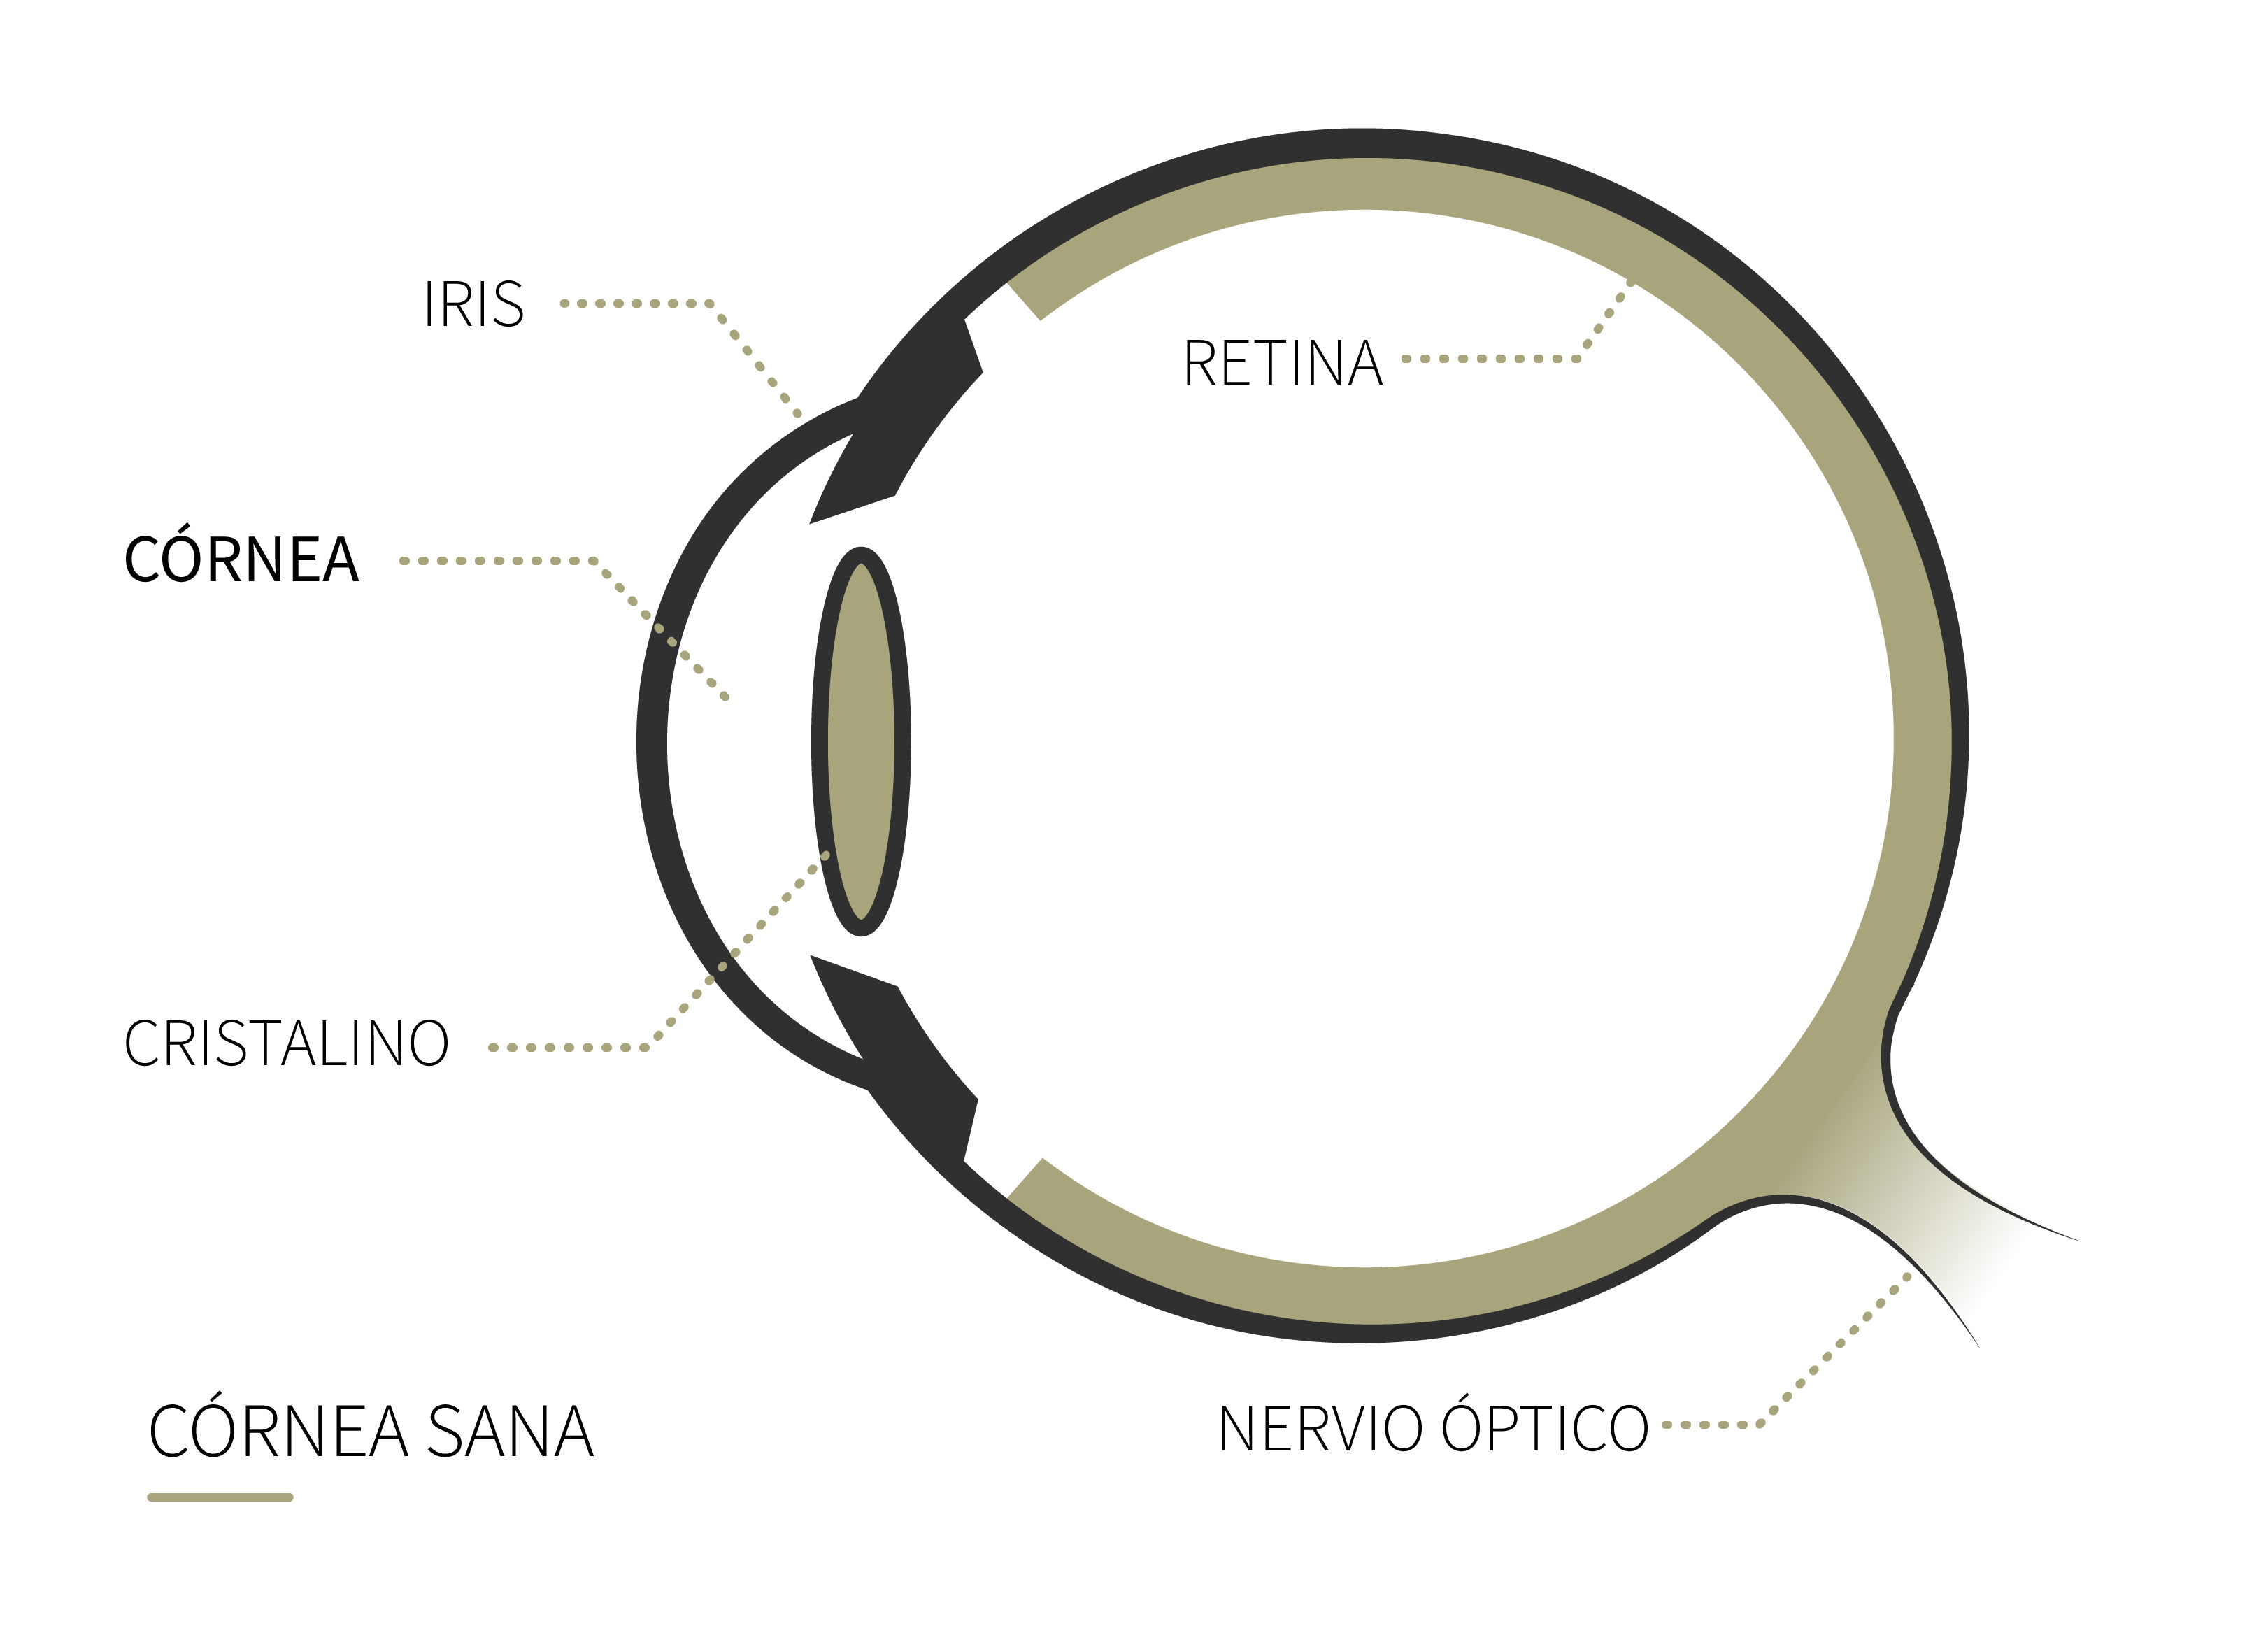
\includegraphics[width=0.49\linewidth]{queratocono_deformacion_a.png}\hfill
            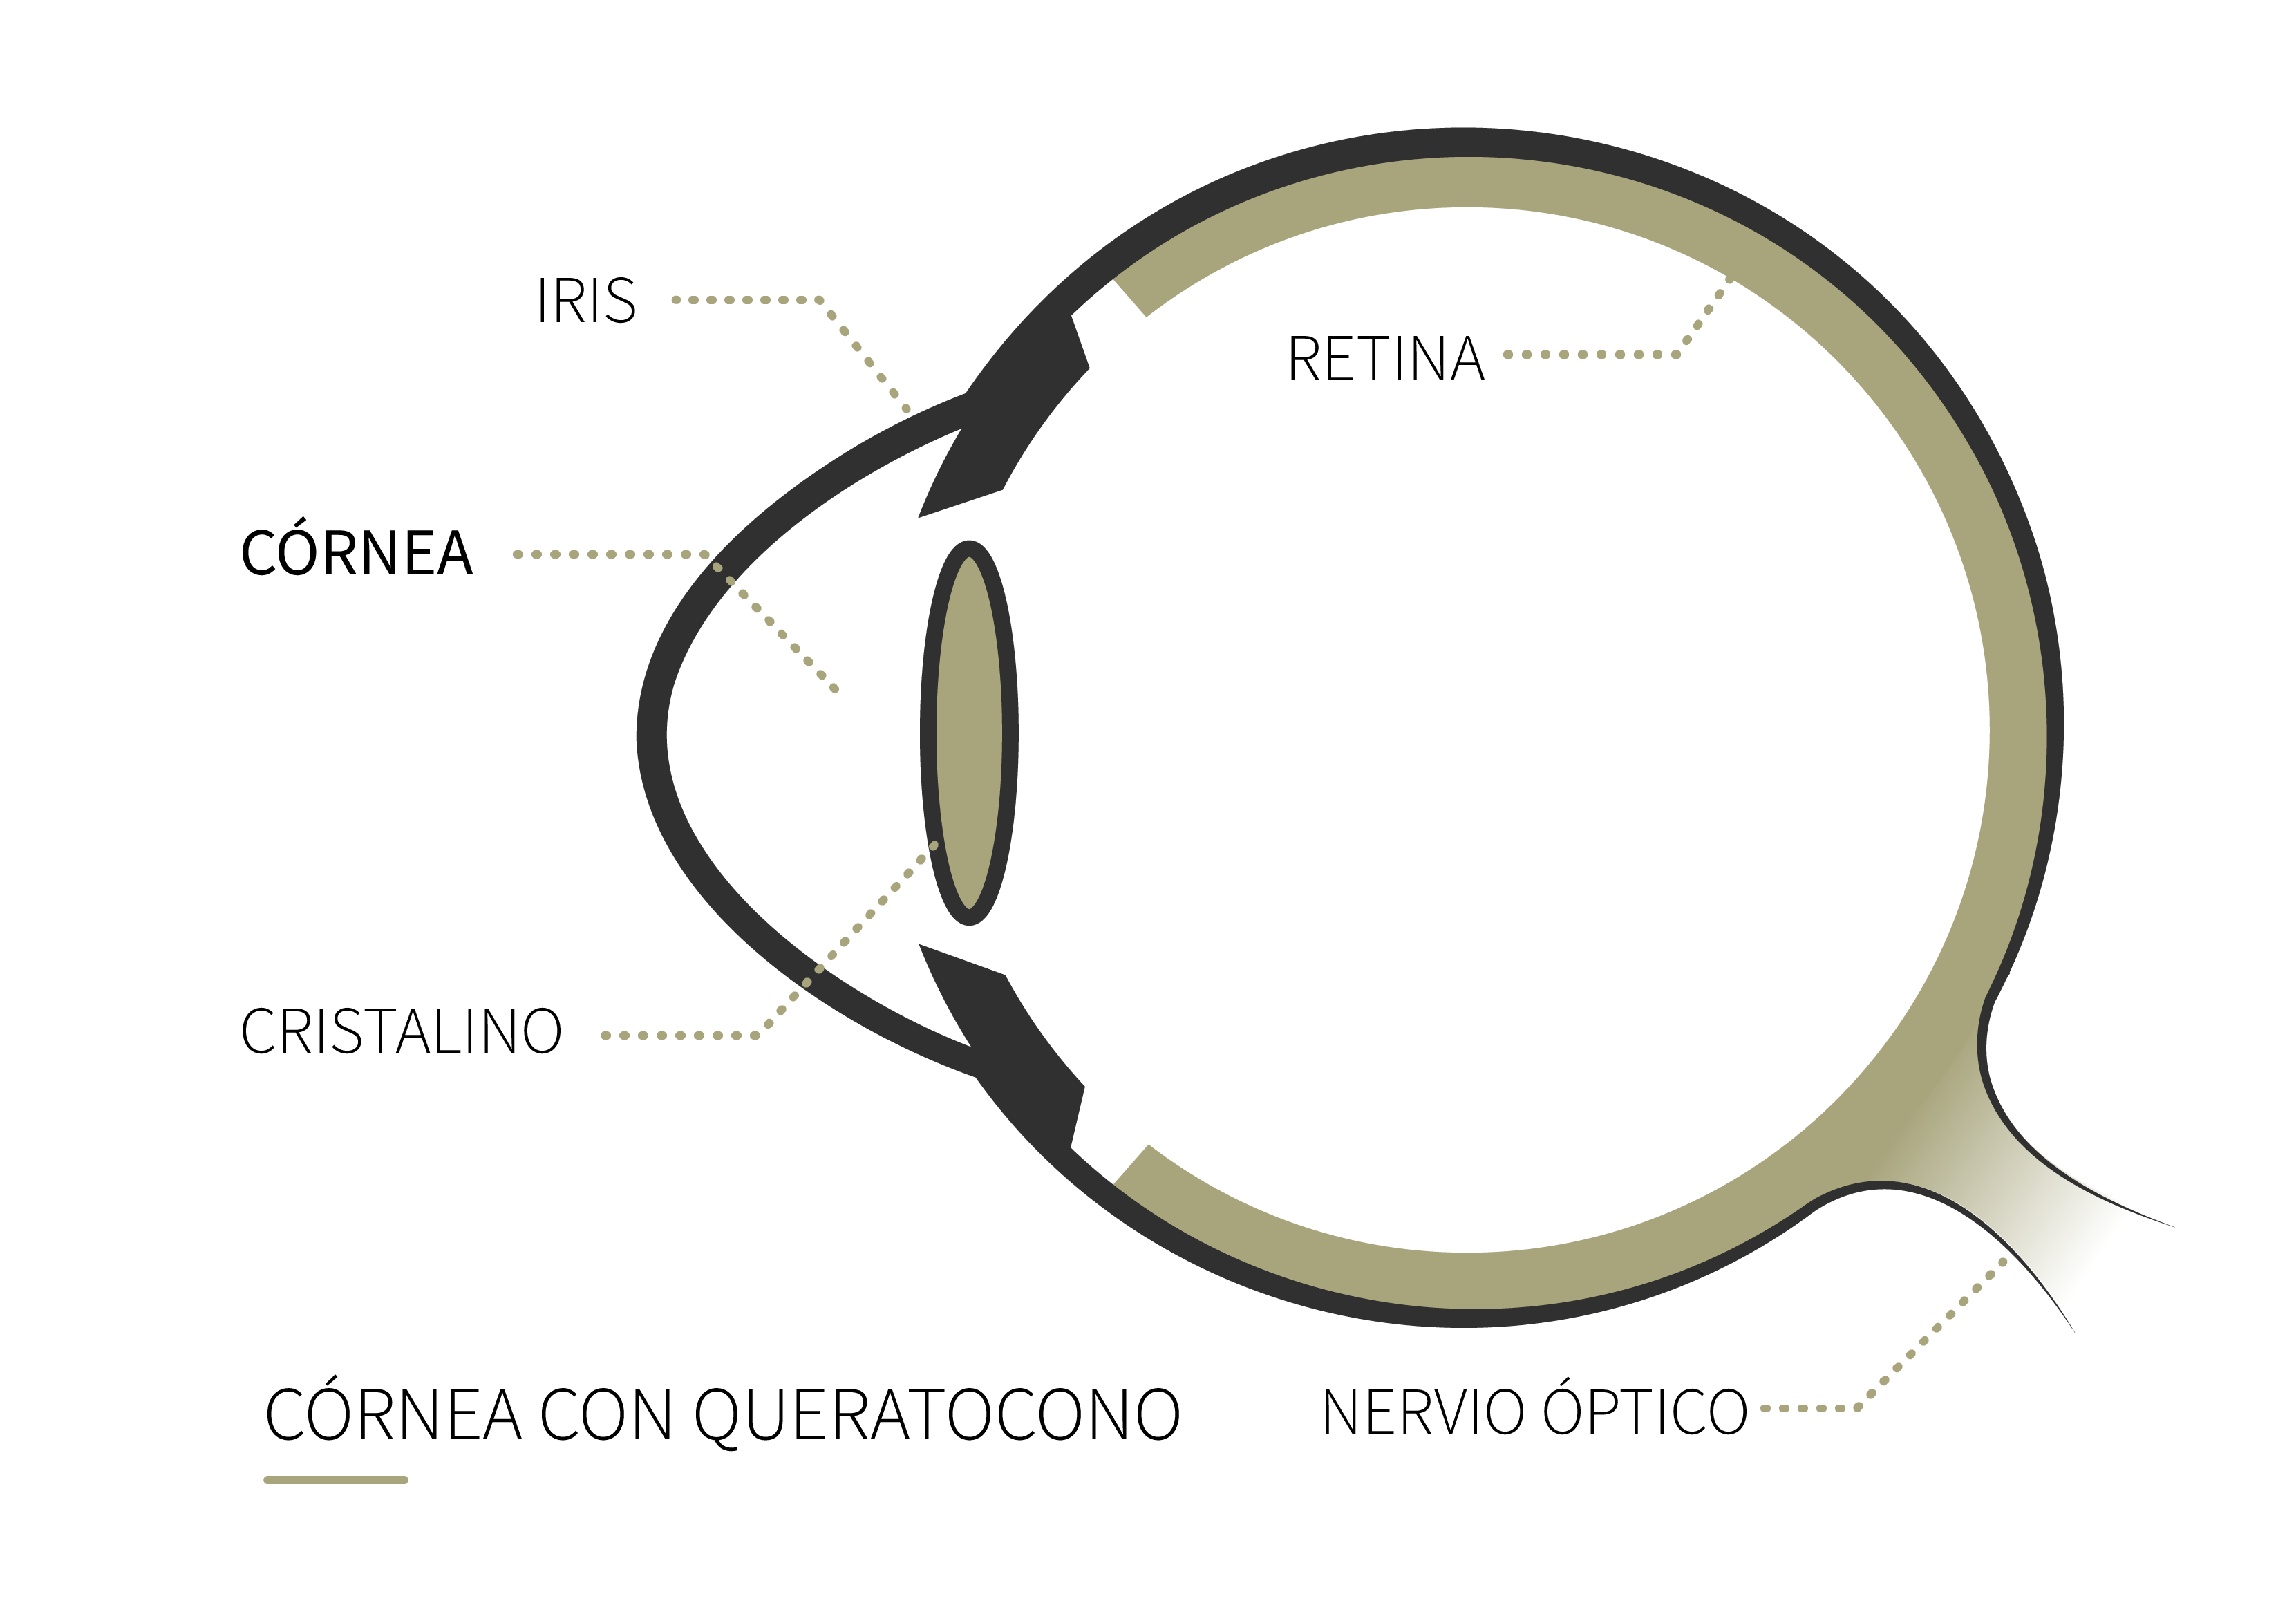
\includegraphics[width=0.49\linewidth]{queratocono_deformacion_b.png}\par
            {\scriptsize Córnea sana \hspace{1.5cm} Córnea con queratocono}
        \end{column}
    \end{columns}
    \idea{El problema no es la enfermedad, es detectarla a tiempo.}
\end{frame}

% ===============================================================
% 2. Qué es KERALYTIX (diagrama de bloques general)
% ===============================================================
\begin{frame}{Qué es KERALYTIX}
    Una herramienta web que le da al oftalmólogo una segunda opinión sobre el estudio de la córnea.
    \vspace{0.1cm}
    \begin{center}
        \begin{tikzpicture}[node distance=0.6cm and 0.9cm]
            \node[caja=3.2cm] (mapas) {\textbf{Mapas de la córnea}\\ \footnotesize los cuatro que exporta el equipo de topografía};
            \node[caja=3.2cm, below=of mapas] (clin) {\textbf{Datos del paciente}\\ \footnotesize edad, sexo, curvatura, espesor};
            \coordinate (medio) at ($(mapas.east)!0.5!(clin.east)$);
            \node[caja=3.2cm, fill=azul!15, very thick, right=1.2cm of medio, anchor=west] (modelo)
                {\textbf{Modelo de IA}\\ \footnotesize analiza imágenes y datos juntos};
            \node[caja=3.2cm, draw=verde, right=of modelo] (informe)
                {\textbf{Informe}\\ \footnotesize normal o queratocono, confianza y mapa de calor};
            \draw[flecha] (mapas.east) -- ++(0.6cm,0) |- (modelo.west);
            \draw[flecha] (clin.east) -- ++(0.6cm,0) |- (modelo.west);
            \draw[flecha] (modelo) -- (informe);
            \node[font=\footnotesize\bfseries, text=gray, above=0.15cm of mapas] {Qué recibe};
            \node[font=\footnotesize\bfseries, text=gray] at (modelo |- {$(mapas.north)+(0,0.4cm)$}) {Qué hace};
            \node[font=\footnotesize\bfseries, text=gray] at (informe |- {$(mapas.north)+(0,0.4cm)$}) {Qué entrega};
        \end{tikzpicture}
    \end{center}
    {\small El mapa de calor marca qué zonas de la córnea llevaron al resultado. La decisión final es siempre del médico.}
\end{frame}

% ===============================================================
% 3. Objetivos
% ===============================================================
\begin{frame}{Objetivos}
    \begin{block}{Objetivo general}
        \small Desarrollar un sistema de soporte a la decisión clínica, basado en IA sobre mapas corneales y datos clínicos,
        para la detección temprana del queratocono y accesible mediante una aplicación web.
    \end{block}
    \vspace{0.3cm}
    \begin{tabla}{colspec = {Q[c,m,0.8cm] X[l,m]}, rows = {font=\small}}
        N.º & Objetivos específicos \\
        1 & Analizar un conjunto de datos público con mapas corneales y variables clínicas. \\
        2 & Construir un modelo de IA que combine mapas y variables para identificar el queratocono. \\
        3 & Integrar una explicación visual de las zonas de la córnea que llevaron a cada resultado. \\
        4 & Desarrollar una aplicación web para cargar estudios y consultar el informe. \\
    \end{tabla}
\end{frame}

% ===============================================================
% 4. Fases y estado actual
% ===============================================================
\begin{frame}{Fases del proyecto y estado actual}
    \begin{center}
        \begin{tikzpicture}[x=1.9cm, y=1cm]
            % Meses
            \foreach \m/\n in {1/Ago, 2/Sep, 3/Oct, 4/Nov, 5/Dic}
                \node[font=\footnotesize, text=gray] at (\m-0.5, 3.3) {\n};
            % Fases
            \fill[verde!70] (0,2.2) rectangle (1,2.8);
            \node[anchor=east, font=\small, align=right] at (-0.1,2.5) {Fase 1: comprensión y\\selección de datos};
            \fill[azul!70] (1,1.2) rectangle (4,1.8);
            \node[anchor=east, font=\small] at (-0.1,1.5) {Fase 2: modelado};
            \fill[gray!40] (3,0.2) rectangle (5,0.8);
            \node[anchor=east, font=\small] at (-0.1,0.5) {Fase 3: aplicación web};
            % Objetivos que cubre cada fase
            \node[font=\scriptsize, text=white] at (0.5,2.5) {Obj. 1};
            \node[font=\scriptsize, text=white] at (2.5,1.5) {Obj. 2 y 3};
            \node[font=\scriptsize] at (4,0.5) {Obj. 4};
            % Hoy
            \draw[rojo, very thick, dashed] (3.3,0) -- (3.3,3.05);
            \node[rojo, font=\footnotesize\bfseries, anchor=south] at (3.3,-0.55) {hoy};
        \end{tikzpicture}
    \end{center}
    \vspace{0.1cm}
    \centering
    {\small\textcolor{verde}{\textbf{\textbullet}} Terminada \quad
     \textcolor{azul}{\textbf{\textbullet}} En curso \quad
     \textcolor{gray!60}{\textbf{\textbullet}} Por empezar}
\end{frame}

% LTeX: enabled=false
% Sección 2: resultados por fase, con evidencias y estado de cada uno

\seccion{Resultados por fase}

% ===============================================================
% 5. Fase 1: selección del conjunto de datos
% ===============================================================
\begin{frame}{Fase 1: selección del conjunto de datos}
    \begin{columns}[T]
        \begin{column}{0.44\textwidth}
            Se seleccionó \textbf{CornOrb}, un conjunto de datos público:
            \begin{itemize}
                \item 1.454 ojos de 744 pacientes.
                \item 5.628 imágenes de mapas corneales.
                \item Cada ojo trae sus mapas y sus datos clínicos juntos, que es lo que necesita un modelo multimodal.
                \item El diagnóstico de cada ojo lo asignaron oftalmólogos.
            \end{itemize}
        \end{column}
        \begin{column}{0.52\textwidth}
            \centering
            {\small\textbf{Qué trae cada ojo}}\par\vspace{0.2cm}
            \begin{tikzpicture}[node distance=0.35cm]
                \node[caja=4.6cm] (m) {\textbf{4 mapas de la córnea}\\ \footnotesize curvatura, elevación delantera, elevación trasera y espesor};
                \node[caja=4.6cm, below=of m] (v) {\textbf{Datos clínicos}\\ \footnotesize edad, sexo, curvatura máxima, espesor, astigmatismo};
                \node[caja=4.6cm, draw=verde, below=of v] (e) {\textbf{Diagnóstico}\\ \footnotesize normal o queratocono};
            \end{tikzpicture}
        \end{column}
    \end{columns}
    \alcanzado{Objetivo 1}
\end{frame}

% ===============================================================
% 6. Fase 1: análisis exploratorio (composición y calidad)
% ===============================================================
\begin{frame}{Fase 1: revisión de los datos}
    \begin{columns}[T]
        \begin{column}{0.48\textwidth}
            \centering
            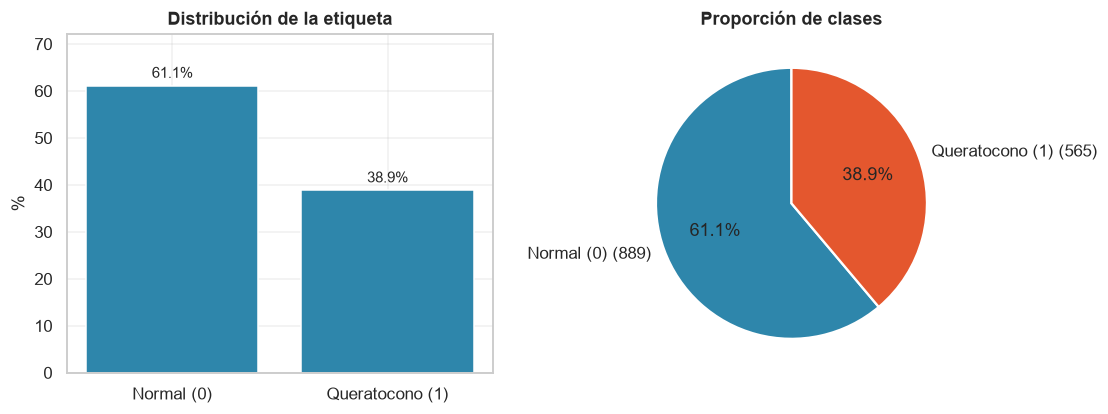
\includegraphics[width=\linewidth]{eda/eda_clases.png}\par
            {\scriptsize 61\% de ojos normales y 39\% con queratocono}
        \end{column}
        \begin{column}{0.48\textwidth}
            \footnotesize
            \textbf{Lo que está bien}
            \begin{itemize}
                \item No faltan datos y cada ojo tiene sus cuatro mapas.
                \item Los ojos de un mismo paciente nunca quedan repartidos entre entrenamiento y prueba. Así el modelo no se evalúa con pacientes que ya conoce.
            \end{itemize}
            \textbf{Lo que hay que corregir}
            \begin{itemize}
                \item 46 ojos medidos más de una vez.
                \item Un código de paciente mal escrito.
                \item Valores imposibles, como una curvatura de 4 cuando lo normal es 44.
            \end{itemize}
        \end{column}
    \end{columns}
    \alcanzado{Objetivo 1}
\end{frame}

% ===============================================================
% 7. Fase 1: qué dicen las variables clínicas
% ===============================================================
\begin{frame}{Fase 1: qué dicen los datos clínicos}
    \begin{columns}[T]
        \begin{column}{0.5\textwidth}
            \centering
            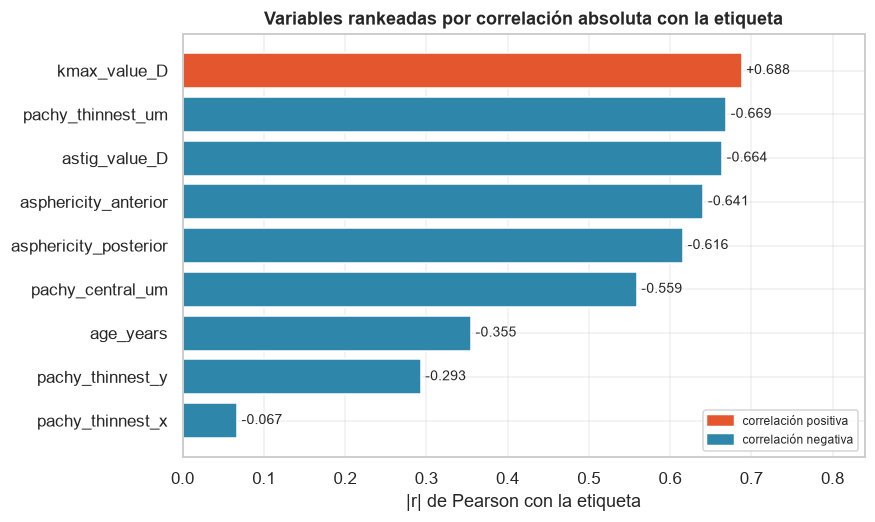
\includegraphics[width=\linewidth]{eda/eda_correlacion.png}\par
            {\scriptsize Cuanto más larga la barra, más se relaciona el dato con el diagnóstico}
        \end{column}
        \begin{column}{0.46\textwidth}
            Los ojos con queratocono tienen:
            \begin{itemize}
                \item Una córnea más curva (53 frente a 44 dioptrías).
                \item Una córnea más delgada (428 frente a 521 micrones).
                \item Más astigmatismo.
            \end{itemize}
            \vspace{0.2cm}
            Coincide con lo que describe la medicina sobre la enfermedad.
        \end{column}
    \end{columns}
    \idea{Los datos clínicos ya separan bastante los dos grupos. Por eso el modelo los combina con las imágenes.}
\end{frame}

% ===============================================================
% 8. Datos locales para la validación
% ===============================================================
\begin{frame}{Datos locales para la validación}
    \begin{columns}[T]
        \begin{column}{0.45\textwidth}
            CornOrb viene de pacientes de Argelia. Para comprobar que KERALYTIX funciona con pacientes de la región, hacen falta estudios locales.
            \begin{itemize}
                \item Se contactaron 9 centros y profesionales de Misiones, Córdoba, Buenos Aires y Perú.
            \end{itemize}
        \end{column}
        \begin{column}{0.51\textwidth}
            \centering
            \begin{tikzpicture}[node distance=0.4cm]
                \node[caja=4.6cm, draw=verde] (a) {\textbf{Contacto con Roberto Albertazzi}};
                \node[caja=4.6cm, draw=verde, below=of a] (b) {\textbf{Charla sobre datos para validar el modelo}};
                \node[caja=4.6cm, fill=azul!15, very thick, below=of b] (c) {\textbf{Trámites legales para la solicitud}\\ \footnotesize estamos acá};
                \node[caja=4.6cm, draw=gray!60, text=gray, below=of c] (d) {Estudios locales anonimizados};
                \draw[flecha] (a) -- (b);
                \draw[flecha] (b) -- (c);
                \draw[flecha, gray!60] (c) -- (d);
            \end{tikzpicture}
        \end{column}
    \end{columns}
    \enproceso{Validación local}
\end{frame}

% ===============================================================
% 9. Fase 2: cómo funciona el modelo (diagrama de bloques)
% ===============================================================
\begin{frame}{Fase 2: cómo funciona el modelo}
    \begin{center}
        \begin{tikzpicture}[node distance=0.5cm and 0.55cm]
            \node[caja=1.9cm] (mapas) {\textbf{Mapas}};
            \node[caja=1.9cm, below=1.1cm of mapas] (datos) {\textbf{Datos clínicos}};
            \node[caja=3cm, right=of mapas] (cnn) {\textbf{Rama de imágenes}\\ \footnotesize aprende a reconocer formas en los mapas};
            \node[caja=3cm, right=of datos] (densa) {\textbf{Rama de datos}\\ \footnotesize analiza los valores numéricos};
            \coordinate (m2) at ($(cnn.east)!0.5!(densa.east)$);
            \node[caja=2.5cm, fill=azul!15, very thick, right=0.6cm of m2, anchor=west] (fus) {\textbf{Fusión}\\ \footnotesize junta lo que encontró cada rama};
            \node[caja=2.6cm, draw=verde, right=of fus] (res) {\textbf{Resultado}\\ \footnotesize normal o queratocono, y confianza};
            \node[caja=2.6cm, draw=verde, above=0.45cm of res] (gc) {\textbf{Mapa de calor}\\ \footnotesize zonas que influyeron};
            \draw[flecha] (mapas) -- (cnn);
            \draw[flecha] (datos) -- (densa);
            \draw[flecha] (cnn.east) -- ++(0.35cm,0) |- (fus.west);
            \draw[flecha] (densa.east) -- ++(0.35cm,0) |- (fus.west);
            \draw[flecha] (fus) -- (res);
            \draw[flecha] (cnn.north) |- node[pos=0.75, above, font=\scriptsize, text=gray] {Grad-CAM} (gc.west);
        \end{tikzpicture}
    \end{center}
    {\small Cada rama se especializa en un tipo de dato y la fusión aprovecha las relaciones entre ambos. Grad-CAM mira la rama de imágenes y marca qué zonas pesaron en el resultado.}
\end{frame}

% ===============================================================
% 10. Fase 2: avance del modelado
% ===============================================================
\begin{frame}{Fase 2: avance del modelado}
    \pendiente{Lo que el compañero tenga presentable del modelo: primera versión entrenada, resultados preliminares, capturas.}
    \enproceso{Objetivos 2 y 3}
\end{frame}

% ===============================================================
% 11. Fase 3: la aplicación web
% ===============================================================
\begin{frame}{Fase 3: la aplicación web}
    \begin{center}
        \begin{tikzpicture}[node distance=0.5cm and 0.65cm]
            \node[caja=2.3cm] (med) {\textbf{Oftalmólogo}\\ \footnotesize desde el navegador};
            \node[caja=2.8cm, right=of med] (front) {\textbf{Página web}\\ \footnotesize carga los estudios y muestra el informe};
            \node[caja=2.8cm, right=of front] (back) {\textbf{Servidor}\\ \footnotesize recibe los estudios y ejecuta el modelo};
            \node[caja=1.9cm, fill=azul!15, very thick, right=of back] (mod) {\textbf{Modelo de IA}};
            \node[caja=2.8cm, below=0.6cm of back] (us) {\textbf{Usuarios y suscripción}\\ \footnotesize quién puede usar el sistema};
            \draw[flecha, <->] (med) -- (front);
            \draw[flecha, <->] (front) -- (back);
            \draw[flecha, <->] (back) -- (mod);
            \draw[flecha, <->] (back) -- (us);
        \end{tikzpicture}
    \end{center}
    \begin{itemize}
        \small
        \item La página web se hace con React y el servidor con FastAPI.
        \item Se trabaja en noviembre y diciembre, superpuesta con el cierre del modelo.
    \end{itemize}
    \porhacer{Objetivo 4}
\end{frame}

% LTeX: enabled=false
% Sección 3: correspondencia entre objetivos y resultados, y próximos pasos

\seccion{Balance}

% ===============================================================
% 12. Objetivos y resultados
% ===============================================================
\newcommand{\etiq}[2]{\fcolorbox{#1}{#1!10}{\textcolor{#1}{\textbf{#2}}}}

\begin{frame}{Lo que nos propusimos y lo que logramos}
    \begin{tabla}{colspec = {Q[c,m,0.7cm] Q[l,m,4.3cm] X[l,m] Q[c,m,2.3cm]},
                  rows = {font=\footnotesize}, rowsep = 1pt}
        Obj. & Qué nos propusimos & Qué logramos & Estado \\
        1 & Analizar un conjunto de datos público & CornOrb seleccionado y revisado, con los datos a corregir identificados & \etiq{verde}{Alcanzado} \\
        2 & Construir el modelo de IA & Diseño definido y comparación de redes base programada, sin resultados todavía & \etiq{azul}{En proceso} \\
        3 & Integrar la explicación visual & Prevista con Grad-CAM, al cierre del modelado & \etiq{gray}{Por empezar} \\
        4 & Desarrollar la aplicación web & Partes y herramientas definidas (React y FastAPI) & \etiq{gray}{Por empezar} \\
        --- & Conseguir datos locales para validar & 9 centros contactados, charla con Roberto Albertazzi y trámites en curso & \etiq{azul}{En proceso} \\
    \end{tabla}
    \vspace{0.2cm}
    \centering
    {\small El avance coincide con el cronograma: la fase 1 está terminada y la fase 2 está en curso.}
\end{frame}

% ===============================================================
% 13. Próximos pasos
% ===============================================================
\begin{frame}{Próximos pasos}
    \begin{columns}[T]
        \begin{column}{0.48\textwidth}
            \begin{block}{Noviembre}
                \begin{itemize}
                    \item Corregir los datos según la revisión.
                    \item Entrenar y evaluar el modelo, priorizando no pasar por alto casos de queratocono.
                    \item Integrar el mapa de calor.
                    \item Empezar la aplicación web.
                \end{itemize}
            \end{block}
        \end{column}
        \begin{column}{0.48\textwidth}
            \begin{block}{Diciembre}
                \begin{itemize}
                    \item Terminar la aplicación web.
                    \item Conectar el modelo con la aplicación.
                    \item Tener el prototipo funcionando de punta a punta.
                \end{itemize}
            \end{block}
            \vspace{0.2cm}
            \begin{block}{En paralelo}
                \begin{itemize}
                    \item Avanzar con los trámites para los datos locales.
                \end{itemize}
            \end{block}
        \end{column}
    \end{columns}
    \idea{Enero queda como reserva por si algo se atrasa.}
\end{frame}


% ===============================================================
% Cierre
% ===============================================================
\begin{frame}[plain]
    \centering\vfill
    {\usebeamercolor[fg]{title}\LARGE\bfseries ¿Preguntas?\par}
    \vspace{0.8cm}
    
\includegraphics[height=2.2cm]{logo_keralytix.png}
    \vfill
\end{frame}

% Diapositivas de respaldo (no suman al total del pie)
\appendix
% LTeX: enabled=false
% Diapositivas de respaldo: solo se muestran si preguntan

% ===============================================================
% R1. Glosario
% ===============================================================
\begin{frame}{Respaldo: glosario}
    \begin{tabla}{colspec = {Q[l,m,4.4cm] X[l,m]}, rows = {font=\footnotesize}, rowsep = 1pt}
        Término & Qué significa \\
        Conjunto de datos (\textit{dataset}) & Estudios ya diagnosticados con los que aprende el modelo. \\
        Multimodal & Que combina distintos tipos de datos, en este caso imágenes y números. \\
        Red neuronal convolucional (CNN) & Tipo de modelo de IA que aprende a reconocer formas en imágenes. \\
        Grad-CAM & Marca qué zonas de la imagen pesaron más en el resultado. \\
        Falso negativo & Un ojo con queratocono que el modelo da como normal. Es el error a evitar. \\
        Sensibilidad & Porcentaje de ojos con queratocono que el modelo detecta. \\
        Validación & Probar el modelo con estudios que nunca vio. \\
    \end{tabla}
\end{frame}

% ===============================================================
% R2. Qué mide el equipo de la córnea
% ===============================================================
\begin{frame}{Respaldo: qué mide el equipo}
    \centering
    \resizebox{\linewidth}{!}{% Esquema de los parámetros corneales (Marco teórico)
% (a) corte de una córnea con queratocono sobre sus esferas de referencia
% (b) vista de frente: ubicación del punto más delgado y orientación en grados
\begin{tikzpicture}[
    font=\small,
    >={Stealth[length=1.8mm]},
    referencia/.style = {dashed, gray!70, thick},
    superficie/.style = {very thick, black!80},
    cota/.style = {<->, thick},
    nota/.style = {font=\footnotesize, align=left, inner sep=1pt,
                   execute at begin node={\setstretch{1}}},
    guia/.style = {thin},
    declare function={
        esfAnt(\x) = sqrt(36 - \x*\x) - 3;          % esfera de referencia anterior
        esfPos(\x) = sqrt(27.04 - \x*\x) - 2.8;     % esfera de referencia posterior
        cono(\x)   = exp(-((\x - 0.8)^2) / 1.6);    % protrusión del cono
        ant(\x)    = esfAnt(\x) + 0.6*cono(\x) - 0.1;
        pos(\x)    = esfPos(\x) + 0.9*cono(\x) - 0.1;
    }
  ]

  % ---------------- (a) Corte de la córnea ----------------
  % Tejido corneal entre ambas superficies
  \fill[blue!10]
    plot[domain=-4:4, samples=120] (\x, {ant(\x)})
    -- plot[domain=4:-4, samples=120] (\x, {pos(\x)}) -- cycle;
  % Esferas de referencia (forma ideal)
  \draw[referencia] plot[domain=-4.2:4.2, samples=80] (\x, {esfAnt(\x)});
  \draw[referencia] plot[domain=-4.2:4.2, samples=80] (\x, {esfPos(\x)});
  % Superficies reales
  \draw[superficie] plot[domain=-4:4, samples=120] (\x, {ant(\x)});
  \draw[superficie] plot[domain=-4:4, samples=120] (\x, {pos(\x)});
  \node[nota] at (-3.2, 2.75) {cara anterior};
  \node[nota] at (-2.0, 1.2) {cara posterior};

  % Zona de 3 mm centrada en el punto más delgado (A y B)
  \draw[orange!80!black, thick, |-|] (-0.15, 4.15) -- (1.75, 4.15)
    node[midway, above=2pt, nota, text=orange!80!black] {zona de 3 mm (A y B)};
  \draw[orange!80!black, densely dotted] (-0.15, 4.15) -- (-0.15, {ant(-0.15)});
  \draw[orange!80!black, densely dotted] (1.75, 4.15) -- (1.75, {ant(1.75)});

  % K max: punto de mayor curvatura de la cara anterior
  \fill[violet] (0.8, {ant(0.8)}) circle (2.2pt);
  \node[nota, text=violet] (lkmax) at (-3.1, 4.3) {\textbf{K max}: punto de mayor\\curvatura de la cara anterior};
  \draw[guia, violet] (lkmax.east) -- (0.75, {ant(0.8)+0.05});

  % Espesor mínimo (C)
  \draw[cota, teal!70!black] (0.8, {pos(0.8)}) -- (0.8, {ant(0.8)});
  \node[nota, text=teal!70!black] (lesp) at (5.6, 3.7) {\textbf{Espesor mínimo (C)}:\\espesor en el punto\\más delgado};
  \draw[guia, teal!70!black] (lesp.west) -- (0.85, {(ant(0.8)+pos(0.8))/2});

  % Elevaciones respecto de las esferas de referencia
  \draw[cota, red!70!black] (1.75, {esfAnt(1.75)}) -- (1.75, {ant(1.75)});
  \draw[cota, red!70!black] (1.75, {esfPos(1.75)}) -- (1.75, {pos(1.75)});
  \node[nota, text=red!70!black] (lelev) at (5.6, 2.1) {\textbf{Elevación} anterior\\y posterior: cuánto\\sobresale cada cara\\de su esfera};
  \draw[guia, red!70!black] (lelev.west) -- (1.8, {(esfAnt(1.75)+ant(1.75))/2});
  \draw[guia, red!70!black] (lelev.west) -- (1.8, {(esfPos(1.75)+pos(1.75))/2});

  % Leyenda
  \draw[referencia] (-4, 0.15) -- ++(0.6, 0) node[right, nota, text=black] {esfera de referencia (forma ideal)};
  \fill[blue!10] (-4, -0.45) rectangle ++(0.6, 0.3);
  \node[nota, right] at (-3.3, -0.3) {tejido corneal};
  \node[font=\small\bfseries] at (0.6, -1.05) {(a) Corte de una córnea con queratocono};
  \node[nota, text=gray] at (0.6, -1.5) {Esquema sin escala: las deformaciones están exageradas.};

  % ---------------- (b) Vista de frente ----------------
  \begin{scope}[shift={(10.6, 2.0)}]
    \fill[blue!6] (0,0) circle (2.1);
    \draw[thick] (0,0) circle (2.1);
    \draw[gray!60] (-2.35,0) -- (2.35,0);
    \draw[gray!60] (0,-2.35) -- (0,2.35);
    \node[nota] at (2.65, 0) {0°};
    \node[nota] at (-2.8, 0) {180°};
    \node[nota] at (0, 2.6) {90°};
    % Dos orientaciones casi iguales: 1° y 179°
    \draw[red!70!black, thick] (0,0) -- (1:2.1) node[pos=0.72, above=1pt, nota, text=red!70!black] {1°};
    \draw[red!70!black, thick, dashed] (0,0) -- (179:2.1) node[pos=0.72, above=1pt, nota, text=red!70!black] {179°};
    % Punto más delgado, su ubicación (x, y) y la zona de 3 mm
    \coordinate (pmd) at (0.55, -0.85);
    \draw[orange!80!black, thick] (pmd) circle (0.7);
    \draw[teal!70!black, densely dotted] (pmd) -- (0.55, 0) node[above, nota, text=teal!70!black] {$x$};
    \draw[teal!70!black, densely dotted] (pmd) -- (0, -0.85) node[left, nota, text=teal!70!black] {$y$};
    \fill[teal!70!black] (pmd) circle (2.2pt);
    \node[nota, align=center] at (0, -2.85) {\textcolor{teal!70!black}{punto más delgado en $(x, y)$}\\\textcolor{orange!80!black}{y zona de 3 mm a su alrededor}};
    \node[nota, align=center, text=red!70!black] at (0, 3.15) {1° y 179° marcan casi\\la misma dirección};
    \node[font=\small\bfseries] at (0, -3.05) [below=8pt] {(b) Vista de frente};
  \end{scope}
\end{tikzpicture}
}
\end{frame}

% ===============================================================
% R3. Detalle del análisis exploratorio
% ===============================================================
\begin{frame}{Respaldo: datos clínicos por grupo}
    \centering
    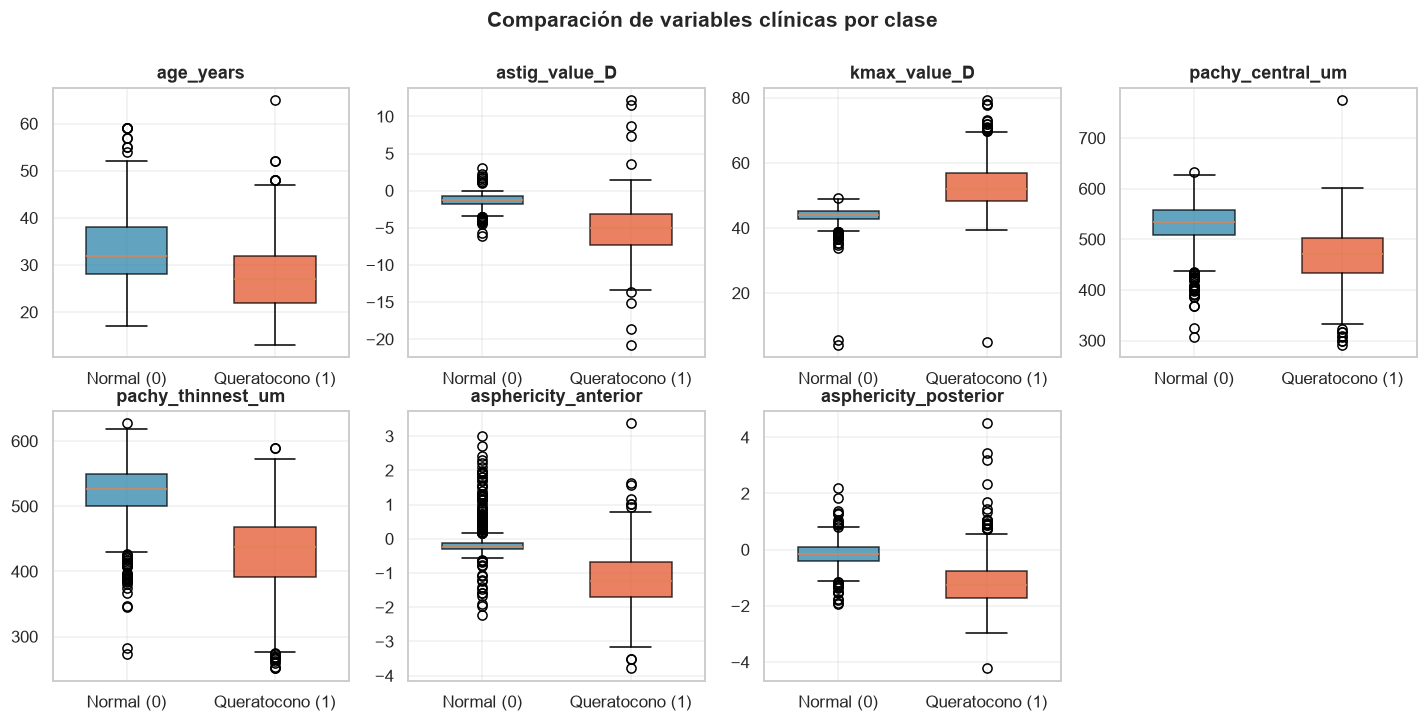
\includegraphics[width=0.82\linewidth]{eda/eda_variables_clinicas.png}\par
    {\small Cada caja muestra la mitad central de los valores de cada grupo, normal y con queratocono.}
\end{frame}


\end{document}
